\subsection{M.PD.17 - Percentuale di test superati}

\begin{figure}[H]
  \centering
  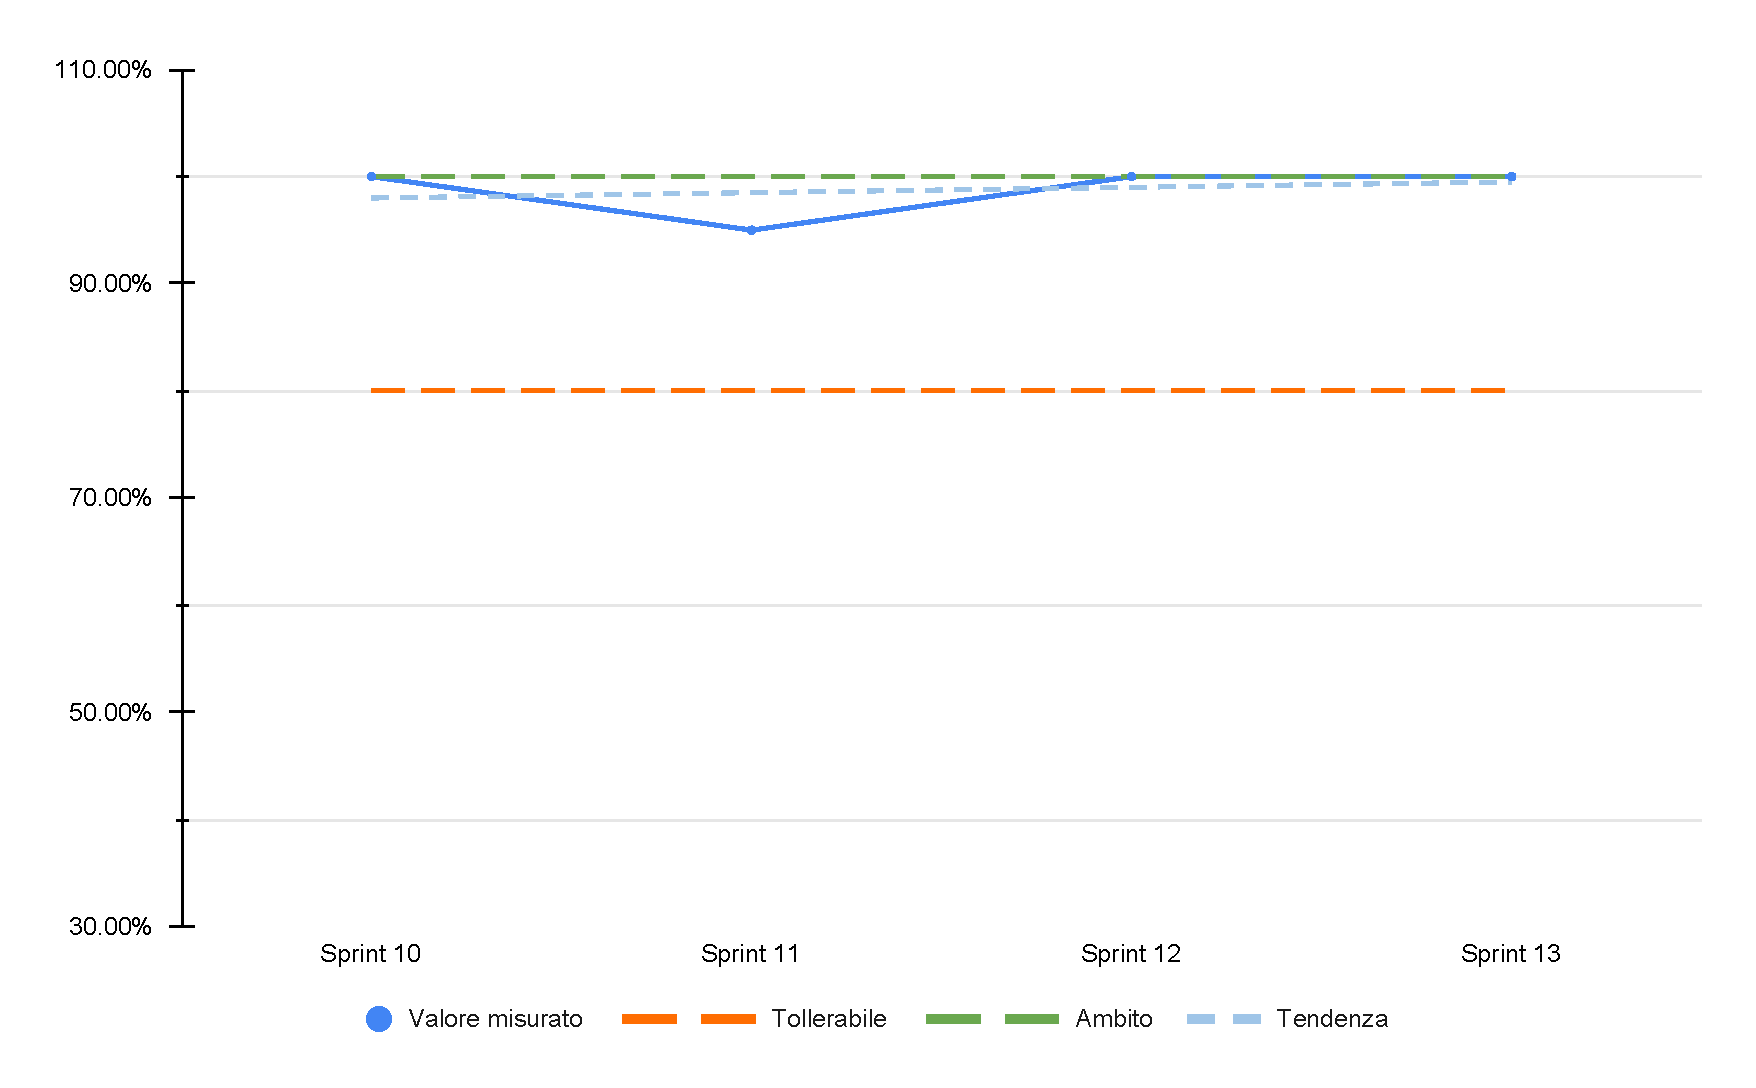
\includegraphics[width=\textwidth]{assets/test_superati.pdf}
  \caption{M.PD.17 - Percentuale di test superati}
\end{figure}

\par A causa dell'inesperienza del team nella scrittura dei test e nell'uso di \glossario{mock} e \glossario{stub}, l'undicesimo sprint si è concluso senza il superamento completo dei test. Dal dodicesimo \glossario{sprint}, le attività di codifica e testing sono state eseguite in parallelo, riducendo significativamente il tasso di errori. Inoltre, il superamento di tutti i test è stato reso una condizione necessaria per chiudere le \glossario{pull request}. Questo ha garantito che i difetti rilevati venissero risolti prima dell'integrazione nell'ambiente condiviso.